\FloatBarrier
\subsection{Other grids and continents}\label{sec:multigrid}

To test whether the findings depend on the British grid, we repeat the experiment on the four further fleets of Table~\ref{tab:fleets}: Europe, the United States, Brazil and a fleet with one site on each of four continents. The last fleet spans time zones from UTC$-8$ to UTC$+12$, so jobs submitted during one region's working day can run in another region's night. For every fleet we retrain the forecaster and tune CARMA, MPC-Protect and the conformal view of MPC on the fleet's own validation weeks (Section~\ref{sec:data}), so no method keeps a setting tuned on Great Britain. Table~\ref{tab:multigrid} and Fig.~\ref{fig:multigrid} summarize the results at $\rho=0.5$, and \appref{app:multigrid} gives all loads.

\begin{table}[!htbp]
\centering
\caption{Results on five grids ($\rho=0.5$, migration allowed; 52 test weeks of 2024). Red.: emission reduction of the oracle relative to ASAP-Local (\%). Columns 3--6: gap to the oracle (\%). Best-base.: gap of the best of Greedy-Spatial, Forecast-Reserve, MPC, MPC-Protect and MPC+conformal minus CARMA's gap (points). Wins: weeks in which CARMA emits less than MPC. Scenario-MPC gap / CARMA gap on the 26 alternating weeks on which Scenario-MPC was run (one trace). Great Britain: main experiment (three traces per week); other fleets: two traces per week.}
\label{tab:multigrid}
\scriptsize\setlength{\tabcolsep}{2.5pt}
\begin{tabular}{lrrrrrrrrr}
\toprule
Fleet & \makecell{Oracle\\red.} & MPC & \makecell{MPC-\\Prot.} & \makecell{MPC+\\conf.} & CARMA & \makecell{Scen.-MPC /\\CARMA} & \makecell{Best-\\base.} & Wins & \makecell{CARMA-\\Perfect} \\
\midrule
\inputtable{../results/table_multigrid.tex}
\bottomrule
\end{tabular}
\end{table}

\begin{figure}[!htbp]
\centering
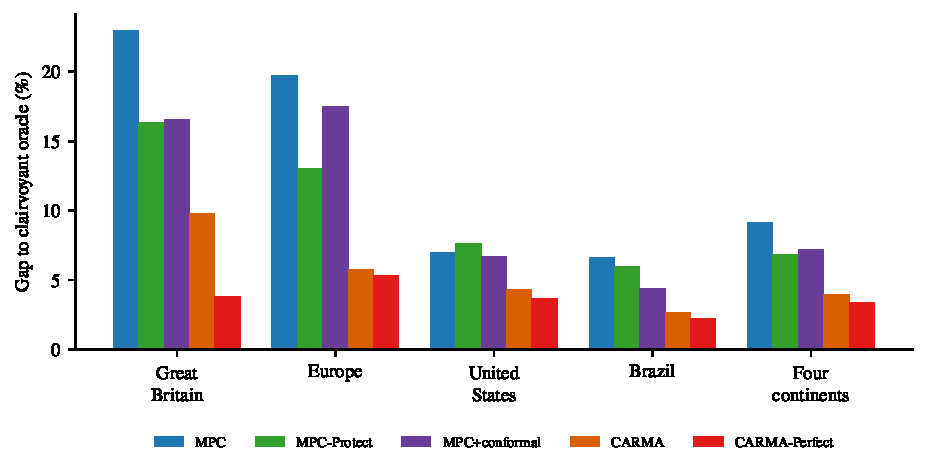
\includegraphics[width=\textwidth]{../figures/fig10_multigrid.pdf}
\caption{Gap to the clairvoyant oracle on five grids ($\rho=0.5$, migration allowed, 52 test weeks; Great Britain with three traces per week, the other fleets with two). Scenario-MPC, which was run on a subset of weeks, is shown in Table~\ref{tab:multigrid}. Bar patterns repeat the legend colors.}
\label{fig:multigrid}
\end{figure}

CARMA has the smallest gap of all implementable policies without a stochastic program on every grid and at every load. At $\rho=0.5$ its gaps are 5.8\% in Europe, 4.3\% in the United States, 2.7\% in Brazil and 4.0\% for the four-continent fleet, against 13.0\%, 6.7\%, 4.4\% and 6.8\% for the best baseline without demand information. CARMA's advantage is 7.3 (95\% block-bootstrap CI 6.2--8.7), 2.4 (2.0--2.9), 1.7 (1.2--2.3) and 2.8 (2.4--3.3) points, and it emits less than MPC in all 52 weeks on each grid. Which baseline is best varies. MPC-Protect is the best baseline in Europe and for the four-continent fleet and MPC+conformal in the United States and Brazil, whereas at $\rho=0.3$ MPC-Protect is worse than plain MPC on all four grids. Over all 15 fleet-load cells the advantage over the best baseline ranges from 1.3 to 7.3 points. It is smaller than in Great Britain (6.3--8.0 points) in the United States and Brazil, and the gap of myopic MPC is correspondingly smaller (7.0\% and 6.6\% at $\rho=0.5$, against 23.0\% in Great Britain). A possible reason is that the sites of these two fleets are closer to each other relative to their mean intensity: the median relative spread between the cleanest and the dirtiest site, $(\max-\min)/\text{mean}$ in 2024, is 1.25 in the United States and 1.27 in Brazil, against 1.71 in Great Britain, 1.80 for the four-continent fleet and 2.06 in Europe, where the nuclear-based French and the coal-based Polish grids are far apart. The advantage broadly follows this spread, but five grids cannot establish a relation. Perfect carbon forecasts would reduce CARMA's gap by a further 0.4--0.6 points at $\rho=0.5$, so the remaining distance to the oracle is mostly due to demand uncertainty. CARMA's late work stays below 0.03\% of work at every load.

The emission reductions follow the same pattern. At $\rho=0.5$ CARMA reduces emissions relative to carbon-agnostic operation by 60.9\% in Europe, 31.8\% in the United States, 35.9\% in Brazil and 54.2\% for the four-continent fleet, compared with 63.0\%, 34.6\%, 37.5\% and 56.0\% for the oracle. These are attributional reductions under production-based intensities and inherit the caveats of the marginal analysis above.

\paragraph{Scenario-MPC} The stochastic lookahead is level with CARMA on three of the new grids. Its gap is 0.09 points above CARMA's in Europe (CI $-0.24$ to 0.42), 0.15 points above it in Brazil (0.01--0.34) and 0.20 points above it for the four-continent fleet ($-0.05$ to 0.55). It is better by 0.44 points in the United States (0.25--0.69), and by 1.0 points in Great Britain on the same subset of weeks. It needs 0.9~s per decision against 33~ms for CARMA, 26--27 times longer. The overall picture from the British experiment therefore holds on other grids: CARMA captures nearly all of the value of demand information at a small fraction of the computing cost of a scenario-based program.

\paragraph{Reversed capacity layout} In all fleets the cleanest site has the least capacity and the smallest share of job origins, as in Great Britain. To check that the result does not depend on this layout, we reverse both assignments, so that the cleanest site is the largest. CARMA's gap is then 6.7\%, 6.0\%, 2.6\% and 3.6\% in Europe, the United States, Brazil and the four-continent fleet, against 18.9\%, 12.4\%, 4.6\% and 6.6\% for the best baseline without demand information (26 alternating weeks, $\rho=0.5$; advantages of 12.1, 6.4, 2.0 and 3.0 points). The oracle's reductions are 61.7\%, 40.7\%, 28.7\% and 46.3\% in this layout, and CARMA's 59.2\%, 37.2\%, 26.9\% and 44.4\%. The ranking of the policies is unchanged.

\paragraph{Forecasts} The forecaster is more accurate than persistence on every grid (mean absolute error of 30.1 against 52.4~gCO$_2$/kWh in Europe, 19.8 against 34.8 in the United States, 7.3 against 12.3 in Brazil and 10.6 against 21.7 for the four-continent fleet), and the adaptively recalibrated upper bounds cover within 0.012 of the target at every level.
